


%\bf{摘要:} 本文提出一种

%\noindent 中文字体(默认宋体)\\
%\fangsong 中文字体(仿宋) \songti 中文字体(宋体) \lishu 中文字体(隶书) \heiti 中文字体(黑体)\\
%\CJKfamily{zhkai} 中文字体(楷书) \CJKfamily{zhyou} 中文字体(幼圆) \CJKfamily{zhyahei} 中文字体(微软雅黑)\\


%\textbf{摘要:}中文摘要中文摘要中文摘要中文摘要中文摘要中文摘要中文摘要中文摘要中文摘要中文摘要中文摘要中文摘要
%
%\textbf{关键词:}关键词1;关键词2;关键词3。

% \textbf{Abstract:} AbstractAbstractAbstractAbstractAbstractAbstractAbstractAbstractAbstractAbstractAbstractAbstractAbstractAbstractAbstract.

% \textbf{keywords: }keywords, keywords, keywords, keywords.
%\setlength{\parindent}{2em} 

%\section{前言}
%
%\label{intro}
%前言前言前言前言前言前言前言前言前言前言前言前言前言前言
%
%前言前言前言前言前言前言前言前言前言前言前言前言前言前言
%
%前言前言前言前言前言前言前言前言前言前言前言前言前言前言
%
%前言前言前言前言前言前言前言前言前言前言前言前言前言前言
%
%前言前言前言前言前言前言前言前言前言前言前言前言前言前言
%
%前言前言前言前言前言前言前言前言前言前言前言前言前言前言
%
%前言前言前言前言前言前言前言前言前言前言前言前言前言前言
%
%前言前言前言前言前言前言前言前言前言前言前言前言前言前言
%
%前言前言前言前言前言前言前言前言前言前言前言前言前言前言
%
%前言前言前言前言前言前言前言前言前言前言前言前言前言前言
%
%
%\begin{figure}[!h]
%	\centering
%	\includegraphics{Fig/Fig1.eps}
%	\caption{无人机}
%	\label{fig:1}     
%\end{figure}

\textbf{\fangsong\xiaosihao 二、立题依据}
% \vspace{-0.30cm}
\begin{ubox}
	\setlength{\parindent}{0em} 
1、研究意义(工程价值)
\vspace{-0.25cm}

2、国内外研究现状(工程应用现状)
\vspace{-0.25cm}

3、主要参考文献及出处
\setlength{\parindent}{2em} 
\section{研究意义}
近几年,随着电子设备集成度不断提高以及动力系统的优化,无人机已经在军事和民用的多种领域得到广泛应用。目前常见的无人机根据其构型大致可以分类为:多旋翼,直升机,固定翼,倾转旋翼,扑翼飞行器,以及本文所研究的涵道式飞行器等。其中,多旋翼飞行器往往由固定于机身主体两个以上的旋翼系统提供主要升力以及操控力矩,由于其结构简单,体积小,垂直起降,易于悬停等特点,在目前的民用场景较为多见。但是其旋翼面积会受到机身体积的制约,而且由于旋翼面积较小,实际上制约着其续航能力。并且暴露的高速转动的旋翼具有一定危险性。随着多旋翼无人机在商业化模式下不断在民用市场普及,被旋翼刮伤的人或物的案例在不断增加。固定翼飞行器由机身发动机提供前进推力,具备固定的机翼或升力面提供升力,由于利用了机翼上的空气动力提供升力,可以实现较远的续航以及较大的载重,但是相比于多旋翼一般需要较大的机身体积来产生足够的升力,起飞和降落往往需要较长的跑道,并且由于需要高速飞行产生升力,固定翼飞机无法长时间悬停以及在小的距离尺寸内灵活机动,这限制了其在城市以及低空环境中的部署。直升机相比于多旋翼而言,只采用一至两个主螺旋桨产生升力,因此旋翼面积更大,续航以及负载超过多旋翼的同时,也兼具垂直起降以及良好的空中机动性能。在开阔地带具备着良好的实用价值,但是同样由于巨大的旋翼的危险性以及较大旋翼面积的要求,在高楼林立的城市低空存在潜在的危险,室内环境中难以派上用场。为了综合多旋翼垂直起降以及固定翼高速长航时的优势,近年来出现了一些倾转旋翼无人机,往往具备固定翼的机翼以及多旋翼的旋翼,但是在旋翼下面安装了倾转机构,可以让升力向上,类似于多旋翼一样完成垂直起降,然后在空中可以转动旋翼,从向上的升力转动为向前的推力,过渡为类似固定翼的飞行模式。这种设计兼具了二者的优势,近年来也得到广泛研究和应用,但是倾转机构设计较为复杂,需要精心设计,往往会带来结构死重,而且旋翼的最佳气动效率难以兼容升力和推力的两种不同飞行状态。另外还有扑翼飞行器,仿照鸟类昆虫等飞行模式,扇动翅膀飞翔,其设计复杂,载重和续航非常有限。
本文所研究的涵道飞行器,是指以涵道风扇构成主要动力来源的无人飞行器。在同样功率消耗下,涵道风扇较同样直径的孤立螺旋桨会产生更大的拉力。同时由于涵道的环括作用,其结构紧凑,气动噪声低,使用安全性好。其应用出现在直升机的涵道尾桨,固定翼飞机的机翼内融合涵道风扇增升装置等。涵道无人飞行器一般将涵道风扇本身作为无人机主体。从结构上大致可以分为三大部分:涵道主体,旋翼和尾部导流板。具有垂直起降,悬停飞行,高速巡航飞行的良好机动能力,体积小巧紧凑。

与其他的无人机相比,涵道无人机具有以下几个特点:
\begin{figure}[H]
	\centering
	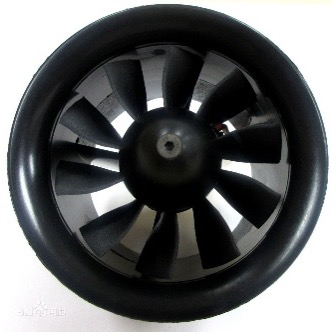
\includegraphics[width=0.4\linewidth]{p1.jpg}
	\caption{一个图片例子}
	\label{fig:main}
\end{figure}

1)机动性能独具特色,适于在城市复杂环境下执行任务。与固定翼无人机相比,涵道式无人机可以在狭小区域内垂直起降,并可以在固定目标上空悬停监视,甚至可以降落到高层建筑物上对地面状况进行观察。

2)结构紧凑,推进效率高。同无人直升机相比,在同等功率消耗下,涵道风扇较同直径的孤立螺旋桨,会产生更大的拉力;而且涵道式无人机结构更加紧凑,前飞时飞行阻力小,飞行姿态更接近于固定翼飞机,因此,飞行速度较同级无人直升机高。

3)噪音低,隐蔽性好。由于螺旋桨位于涵道内,其气动噪声的传播受到了涵道壁的阻挡,这在一定程度上降低了无人机噪音的强度和传播距离;同样由于发动机被涵道环扩,涵道对发动机热辐射的阻挡也可以降低整机的热辐射特性,从而使得涵道无人机具有更好的隐蔽性。

涵道无人机因为其独特的应用性能而备受瞩目,成为当今无人机研究领域中的热点之一,但是其发展仍处在上升的阶段,与之相应的结构、气动以及控制理论和方法引起了近年来的广泛研究,依然存在着许多问题: 

1)就涵道风扇技术而言,虽然早在20世纪50年代人们就已进行了较为充分的理论与实验研究,但是研究对象是作为常规布局飞行器动力装置的涵道发动机,对于作为飞行器主体的涵道风扇的结构特点、微小型涵道风扇在低速大攻角状态下的气动特性以及环形机翼气动特性的研究都少有成熟的理论和可靠的结论;

2)低雷诺数下的剧烈升阻比下降和升力曲线非线性变化,将会对微小型涵道式飞行器的气动性能和控制带来非常不利的影响,因此,如何提高升力、降低阻力、消除气动力非线性变化影响将是涵道无人机气动研究中要解决的主要问题;

3)同涵道发动机不同,涵道式飞行器在涵道本体尾部通常装有姿态控制组件,其结构、搭配方式和组合方法多种多样;处于涵道与姿控组件复合流场中的舵片组合,其气动特性的好坏是能否实现飞行器灵活机动的关键,如何克服这些技术问题、为涵道无人机的广泛应用铺平道路,仍然是当前涵道无人机研究领域的工作重点。

本文将会在以往研究的基础上,自主设计涵道无人机,并且对其空气动力学特性,模型建立,以及控制器设计等方面对其进行分析讨论。并且最终用实际飞行实验对本文所提出的无人机设计以及控制效果进行验证。

\section{国内外研究现状}
\subsection{国外单涵道研究现状}
国外涵道风扇无人飞行器的研究从 20 世纪 80 年代就已兴起,尤其以美国研究技术最为领先。当时,针对美国海军陆战队的(Exploratory  Development  Surveillance Program)启动了空中远程遥控装置(Airborne  Remotely  Operated  Device  ,AROD),用于短期的空中监视任务[3]。该平台经历了一代和二代两个阶段,后期作为低空遥控机器人先期演示验证项目的一部分进行开发。
\begin{figure}[H]
	\centering
	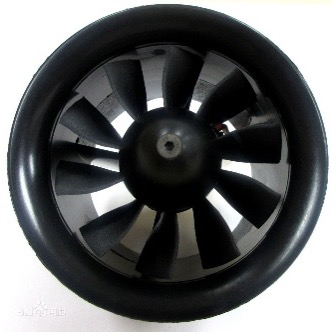
\includegraphics[width=0.4\linewidth]{p1.jpg}
	\caption{一个图片例子}
	\label{fig:main}
\end{figure}
1992 年,美国启动了多用途安全与监视任务平台 (Multipurpose  Security  and Surveillance Mission Platform)。该平台采用 Sikorsky 公司 Cypher 方案。Cypher 飞行平台采用共轴双旋翼涵道式布局,机体扁平,涵道直径比较小,在平飞的时候可以提供一部分升力,平台的飞行姿态控制是通过螺旋桨的周期变距来实现的[4]。

Cypher2 型无人机在 1 型的基础上增加前行涵道风扇和水平翼面,在结构改动不大的情况下,通过前行涵道风扇的推力,和水平翼面的增升稳定作用,可以达到提高飞行速度的目的,使得无人机兼具了垂直起降和快速飞行两方面优点。但是该方案增加了无人机系统的机构复杂性,导致无人机系统可控性,稳定性,续航时间降低。
\begin{figure}[H]
	\centering
	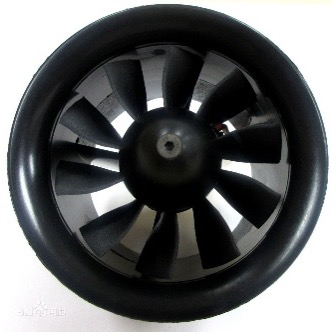
\includegraphics[width=0.4\linewidth]{p1.jpg}
	\caption{一个图片例子}
	\label{fig:main}
\end{figure}
美国在二十世纪初启动了 OAV 竞标计划。OAV  I 采用了联合宇航公司的 29 英寸 i-STAR 涵道风扇无人机,该机开发和集成了 MEMS(Micro-Electro- Mechanical Systems)系统,使得该无人机更利于控制,并且对它的风扇进行了改进.改良了它的空气动力学性能。
OAV II 使用了 Honeywell 公司的涵道风扇式微型无人机 T-hawk,这种微型无人机已经选做 FCS  I 级 UAV该涵道飞行器尺寸上稍微大些,载重量提高,有效载荷可达 9kg。该无人机使用一个 30kg 的重油发动机来驱动,续航时间达到2h,飞行半径 16km。
\begin{figure}[H]
	\centering
	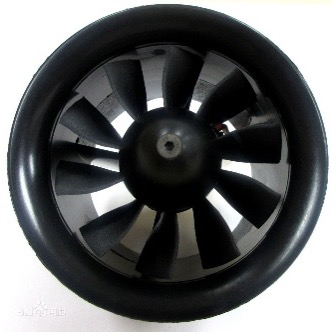
\includegraphics[width=0.4\linewidth]{p1.jpg}
	\caption{一个图片例子}
	\label{fig:main}
\end{figure}

\subsection{国内单涵道研究现状}
\begin{table}[H]
	\centering
	\small
	\caption{数值}
	\resizebox{!}{!}{\begin{tabular}{cccc}
			\hline 
			参数符号 & 数值                & 参数符号 & 数值                 \tabularnewline
			\hline 
			$I_x$   & $054593$ 		     & $I_y$   & $0.017045         $ \tabularnewline
			$l_1$   & $0.0808\,\text{m}$ & $l_2$   & $0.175\,\text{m}  $ \tabularnewline 
			$l_4$   & $0.2415\,\text{m}$ & $l_5$   & $0.1085\,\text{m} $ \tabularnewline
			\hline 
	\end{tabular}}
\end{table}
国内较早对小型涵道飞行器进行研究的单位是南京航空航天大学。2003 年,南航率先研制出涵道式共轴双桨飞行器。这种飞行器与 Cypher 无人机相似[6]。

2005 年,盛世特种飞行公司、哈尔滨工业大学以及航天科工集团联合发展了“跳棋”涵道飞行器[7][8],该种飞机与 I-star 涵道飞机极为相似。上述三方又于 2008 年推出了新一代涵道飞行器,该飞行器内径 1.2 米,重大 10 千克,可在 50~1000 米高度飞行,航时 40 分钟。动力采用活塞发动机。控制方法类似于 I-star。
中航工业集团研制的“旋风侦察兵”涵道无人机。该款飞行器可有多重巡航模式,起飞重量达 8 千克,最大升限达 3000 米,可连续飞行 30 分钟左右。

2014 年 9 月,北京无人机航展展出了南京航空航天大学研制的共轴双桨涵道飞行器,该种涵道飞行器为民用,由共轴安装的两个电机驱动螺旋桨提供飞行动力,绕涵道周围的四个电机驱动小旋翼通过调节自身升力控制飞行器姿态。飞行器最大尺寸达到 1700mm,空机重 8kg,最大飞行器速度达到 70km/h,续航时间 20min。
符号约定符号约定符号约定符号约定符号约定符号约定
\begin{table}[H]
	\centering
	\small
	\caption{数值}
	\resizebox{!}{!}{\begin{tabular}{cccc}
			\hline 
			参数符号 & 数值                & 参数符号 & 数值                 \tabularnewline
			\hline 
			$I_x$   & $054593$ 		     & $I_y$   & $0.017045         $ \tabularnewline
			$l_1$   & $0.0808\,\text{m}$ & $l_2$   & $0.175\,\text{m}  $ \tabularnewline 
			$l_4$   & $0.2415\,\text{m}$ & $l_5$   & $0.1085\,\text{m} $ \tabularnewline
			\hline 
	\end{tabular}}
\end{table}
\begin{equation}
	\begin{aligned}
		a &= b + c \\
		d &= e + f + g \\
		h + i &= j + k \\
		l + m &= n
	\end{aligned}
\end{equation}
符号约定符号约定符号约定符号约定符号约定符号约定
\begin{equation}
	\begin{aligned}
		a &= b + c \\
		d &= e + f + g \\
		h + i &= j + k \\
		l + m &= n
	\end{aligned}
\end{equation}
符号约定符号约定符号约定符号约定符号约定符号约定
\begin{equation}
	\begin{aligned}
		a &= b + c \\
		d &= e + f + g \\
		h + i &= j + k \\
		l + m &= n
	\end{aligned}
\end{equation}
\section{主要参考文献及出处}
\setstretch{1.4} % 设置参考文献行间距,可以按需要调整
\printbibliography[heading=none]
\end{ubox}

\textbf{\fangsong\xiaosihao 三、研究方案}
% \vspace{-0.30cm}
\begin{ubox}
\setcounter{section}{0}
\setcounter{figure}{0}
\setcounter{table}{0}
\setlength{\parindent}{0em} 
1. 研究目标、研究内容及拟解决的关键问题
\vspace{-0.25cm}

2. 拟采取的研究方法、技术路线及可行性分析
\vspace{-0.25cm}

3. 创新之处
\setlength{\parindent}{2em} 
\section{研究目标、研究内容及拟解决的关键问题}
控制器设计控制器设计控制器设计控制器设计控制器设计控制器设计控制器设计控制器设计
\subsection{研究目标}
符号约定符号约定符号约定符号约定符号约定符号约定
\setcounter{equation}{0} 
\begin{equation}
	\begin{aligned}
		a &= b + c \\
		d &= e + f + g \\
		h + i &= j + k \\
		l + m &= n
	\end{aligned}
\end{equation}
符号约定符号约定符号约定符号约定符号约定符号约定
\begin{figure}[H]
	\centering
	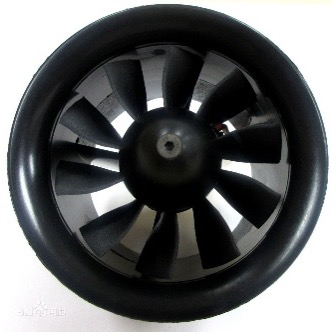
\includegraphics[width=0.4\linewidth]{p1.jpg}
	\caption{一个图片例子}
	\label{fig:main}
\end{figure}

\begin{equation}
	\begin{aligned}
		a &= b + c \\
		d &= e + f + g \\
		h + i &= j + k \\
		l + m &= n
	\end{aligned}
\end{equation}
符号约定符号约定符号约定符号约定符号约定符号约定
\begin{equation}
	\begin{aligned}
		a &= b + c \\
		d &= e + f + g \\
		h + i &= j + k \\
		l + m &= n
	\end{aligned}
\end{equation}
\subsection{研究内容}
符号约定符号约定符号约定符号约定符号约定符号约定
\begin{equation}
	\begin{aligned}
		a &= b + c \\
		d &= e + f + g \\
		h + i &= j + k \\
		l + m &= n
	\end{aligned}
\end{equation}
\subsection{拟解决的关键问题}
符号约定符号约定符号约定符号约定符号约定符号约定
\setcounter{equation}{0} 
\begin{equation}
	\begin{aligned}
		a &= b + c \\
		d &= e + f + g \\
		h + i &= j + k \\
		l + m &= n
	\end{aligned}
\end{equation}
\section{拟采取的研究方法、技术路线及可行性分析}
\subsection{拟采取的研究方法}
飞行试验飞行试验飞行试验飞行试验飞行试验飞行试验飞行试验飞行试验飞行试验飞行试验飞行试验
符号约定符号约定符号约定符号约定符号约定符号约定
\begin{table}[H]
	\centering
	\small
	\caption{数值}
	\resizebox{!}{!}{\begin{tabular}{cccc}
			\hline 
			参数符号 & 数值                & 参数符号 & 数值                 \tabularnewline
			\hline 
			$I_x$   & $054593$ 		     & $I_y$   & $0.017045         $ \tabularnewline
			$l_1$   & $0.0808\,\text{m}$ & $l_2$   & $0.175\,\text{m}  $ \tabularnewline 
			$l_4$   & $0.2415\,\text{m}$ & $l_5$   & $0.1085\,\text{m} $ \tabularnewline
			\hline 
	\end{tabular}}
\end{table}
\begin{figure}[H]
	\centering
	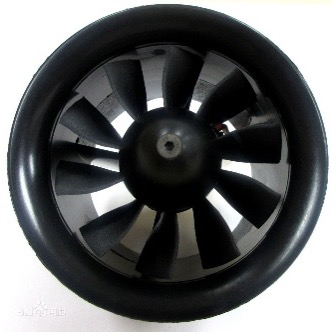
\includegraphics[width=0.4\linewidth]{p1.jpg}
	\caption{一个图片例子}
	\label{fig:main}
\end{figure}
\subsection{技术路线}
\begin{equation}
	\begin{aligned}
		a &= b + c \\
		d &= e + f + g \\
		h + i &= j + k \\
		l + m &= n
	\end{aligned}
\end{equation}
符号约定符号约定符号约定符号约定符号约定符号约定
\begin{equation}
	\begin{aligned}
		a &= b + c \\
		d &= e + f + g \\
		h + i &= j + k \\
		l + m &= n
	\end{aligned}
\end{equation}
\subsection{可行性分析}
符号约定符号约定符号约定符号约定符号约定符号约定
\begin{equation}
	\begin{aligned}
		a &= b + c \\
		d &= e + f + g \\
		h + i &= j + k \\
		l + m &= n
	\end{aligned}
\end{equation}
\section{创新之处}
结论结论结论结论结论结论结论结论结论结论结论结论结论结论结论结论结论结论结论结论结论结论结论结论结论结论结论结论结论结论结论结论结论结论结论结论结论结论结论结论结论结论结论结论结论结论结论结论结论结论

%\begin{table}{H}
%	\caption{\label{TDF_para}涵道模型参数}
%	\centering
%	\small 
%	
%	\begin{tabular}{cccc}
%		\hline 
%		参数符号 & 数值                & 参数符号 & 数值                 \tabularnewline
%		\hline 
%		$I_x$   & $054593$ 		     & $I_y$   & $0.017045         $ \tabularnewline
%		$l_1$   & $0.0808\,\text{m}$ & $l_2$   & $0.175\,\text{m}  $ \tabularnewline 
%		$l_4$   & $0.2415\,\text{m}$ & $l_5$   & $0.1085\,\text{m} $ \tabularnewline
%		\hline 
%	\end{tabular}
%
%\end{table}
\begin{table}[H]
	\centering
    \small
    \caption{数值}
	\resizebox{!}{!}{\begin{tabular}{cccc}
		\hline 
		参数符号 & 数值                & 参数符号 & 数值                 \tabularnewline
		\hline 
		$I_x$   & $054593$ 		     & $I_y$   & $0.017045         $ \tabularnewline
		$l_1$   & $0.0808\,\text{m}$ & $l_2$   & $0.175\,\text{m}  $ \tabularnewline 
		$l_4$   & $0.2415\,\text{m}$ & $l_5$   & $0.1085\,\text{m} $ \tabularnewline
		\hline 
	\end{tabular}}
\end{table}
结论结论结论结论结论结论结论结论结论结论结论结论结论结论结论结论结论结论结论结论结论结论结论结论结论结论结论结论结论结论结论结论结论结论结论结论结论结论结论结论
\end{ubox}

\textbf{\fangsong\xiaosihao 四、研究条件与基础}
% \vspace{-0.30cm}
\begin{ubox}
	\setcounter{section}{0}
	\setcounter{figure}{0}
	\setcounter{table}{0}
	\setlength{\parindent}{0em} 
	1. 相关的研究工作积累
	\vspace{-0.25cm}
	
	2. 已具备的研究条件,尚缺少的研究条件和拟解决的途径
	\vspace{-0.25cm}
	
	3. 本人已取得的主要成果
	
	\setlength{\parindent}{2em} 
	\section{相关的研究工作积累}
	控制器设计控制器设计控制器设计控制器设计控制器设计控制器设计控制器设计控制器设计结论结论结论结论结论结论结论结论结论结论结论结论结论结论结论结论结论结论结论结论结论结论结论结论结论结论结论结论结论结论结论结论结论结论结论结论结论结论结论结论结论结论结论结论结论结论结论结论结论结论结论结论结论结论结论结论结论结论结论结论结论结论结论结论结论结论结论结论结论结论结论结论结论结论结论结论结论结论结论结论结论结论结论结论结论结论结论结论结论结论结论结论结论结论结论结论结论结论结论结论结论结论结论结论结论结论结论结论结论结论结论结论结论结论结论结论结论结论结论结论
	\section{已具备的研究条件,尚缺少的研究条件和拟解决的途径}
	结论结论结论结论结论结论结论结论结论结论结论结论结论结论结论结论结论结论结论结论结论结论结论结论结论结论结论结论结论结论结论结论结论结论结论结论结论结论结论结论
\subsection{已具备的研究条件}
结论结论结论结论结论结论结论结论结论结论结论结论结论结论结论结论结论结论结论结论结论结论结论结论结论结论结论结论结论结论结论结论结论结论结论结论结论结论结论结论
\subsection{尚缺少的研究条件}
结论结论结论结论结论结论结论结论结论结论结论结论结论结论结论结论结论结论结论结论结论结论结论结论结论结论结论结论结论结论结论结论结论结论结论结论结论结论结论结论
\subsection{拟解决的途径}
结论结论结论结论结论结论结论结论结论结论结论结论结论结论结论结论结论结论结论结论结论结论结论结论结论结论结论结论结论结论结论结论结论结论结论结论结论结论结论结论
\section{本人已取得的主要成果}
本人已取得的主要成果
\end{ubox}
